\chapter{Teoremas de Existencia y Unicidad}
\addtocounter{ejemplo_cont}{1}

\section{Sistemas de Ecuaciones Diferenciales}
\subsection{Definición y ejemplos}
Un \emph{sistema de ecuaciones diferenciales de primer orden} es un conjunto  de ecuaciones que relacionan una variable independiente, digamos $x$, un conjunto de variables dependientes, digamos $y_1(x),\ldots,y_n(x)$, y sus derivadas respecto a $x$. A las ecuaciones diferenciales con una incognita y una ecuación las denominaremos \emph{ecuaciones escalares}.

\begin{definicion} Un sistema de ecuaciones diferenciales es una conjunto de ecuaciones de la forma
\begin{equation}\label{eq:sist_ecua}
\left\{
\begin{split}
 \frac{dy_1}{dx}(x)&=f_1(x,y_1(x),\ldots,y_n(x))\\
  \frac{dy_2}{dx}(x)&=f_2(x,y_1(x),\ldots,y_n(x))\\
       &\,\,\vdots                                   \\
 \frac{dy_n}{dx}(x)&=f_n(x,y_1(x),\ldots,y_n(x))\\
\end{split}\right.,
\end{equation}
donde $f_j:[a,b]\times\rr^n\to\rr$, $j=1,\ldots,n$, son funciones.

Una manera alternativa y compacta de denotar un sistema se logra introduciendo las funciones $y=(y_1,\ldots,y_n)$  y $f=(f_1,\ldots,f_n)$. Entonces $y:[a,b]\to\rr^n$ es una función con valores en $\rr^n$ y $f:[a,b]\times \rr^n\to\rr^n$ es un campo vectorial dependiente de $x$. Con estas notaciones el sistema se escribe:
\begin{equation}\label{eq:sist_ecua_comp}
 y'(x)=f(x,y(x)).
\end{equation}

\end{definicion}






\begin{ejemplo} \textbf{Ecuación del péndulo.} Si $x(t)$ es el ángulo que forma un péndulo, de longitud $l$, con la vertical en el tiempo $t$ y $v(t)=x'(t)$, entonces $x(t)$ y$v(t)$ deben satisfacer el siguiente sistema de  ecuaciones:
\begin{equation}\label{eq:sist_pend}
\left\{
\begin{split}
 x'(t)&=v(t)\\
  v'(t)&=-\frac{g}{l}\sen(x(t)).\\
\end{split}\right.
\end{equation}


\end{ejemplo}


\begin{ejemplo} \textbf{Sistemas de ecuaciones de Lotka-Volterra}
 En 1925 y 1926, Alfred J. Lotka y Vito Volterra respectivamente, introdujeron
 las \href{https://es.wikipedia.org/wiki/Ecuaciones_Lotka%E2%80%93Volterra}{ecuaciones de Lotka-Volterra}\link. \marginpar{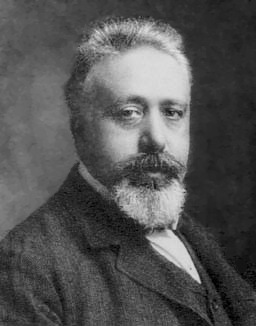
\includegraphics[scale=.28]{imagenes/Vito_Volterra.jpg}\\
 Vito Volterra (1860-1940)}  Se trata de un sistema de dos ecuaciones diferenciales de primer orden que se usan para describir dinámicas de sistemas biológicos en el que dos especies interactúan, una como presa y otra como depredador. Se definen como:
\begin{equation}\label{eq:lotka_volterra}
\left\{
\begin{split}
 x'(t) &= x(t) ( \alpha − \beta  y(t) )\\
  y'(t)&=-y(t)(\gamma-\delta x(t))\\
\end{split}\right.
\end{equation}
La variable $y$ representa el número de individuos de algún predador (por ejemplo, un lobo) y $x$ es el número de sus presas (por ejemplo, conejos), $t$ representa el tiempo; y  $\alpha,\beta,\gamma$ y $\delta$ son parámetros (positivos)

\end{ejemplo}


\subsection{Sistemas de ecuaciones y ecuaciones de orden superior}

\emph{Es posible convertir el sistema \eqref{eq:sist_ecua} de $n$-ecuaciones diferenciales de primer orden  en una ecuación escalar de orden $n$
\begin{equation}\label{eq:orden_n}
y^{(n)}=f(x,y,y',\ldots,y^{(n-1)}).
\end{equation}
y viceverza.}

Para justificar la aseveración anterior supongamos que $y=y(x)$ resuelven  \eqref{eq:orden_n} y escribamos:
\[y_1=y,\, y_2=y',\,y_3=y'',\ldots, y_{n}=y^{(n-1)}.\]
Entonces notar que
\begin{equation}\label{eq:sist_ecua_conv}
\left\{
\begin{array}{l l l}
 y_1'(x)&=y_2(x)\\
  y_2'(x)&=y_3(x)\\
       &\,\,\vdots\\
  y_{n-1}'(x)&=y_n(x)\\
 y_n'(x)&=f(x,y_1(x),\ldots,y_n(x))\\
\end{array}\right.,
\end{equation}

Reciprocamente, supongamos que $y_1,\ldots,y_n$ resuelven \eqref{eq:sist_ecua}. Por simplicidad vamos a suponer que las $f_j$ son independientes de $x$, el procedimiento general sigue las mismas líneas que el caso que discutimos aquí. Se toma $y=y_n$ (podríamos usar cualquier $y_j$, $j=1,\ldots,n$). Ahora derivamos sucesivamente $n$-veces respecto a $x$ la ecuación para $y_n$,  y reemplazamos cada derivada $y_j'$ por $f_j$ (vamos a omitir los argumentos de $f_j$ que son en todos los casos $(y_1,\ldots,y_n)$):

\[%\label{eq:sist_ecua_conv}
\begin{array}{c c c}
y_n'(x) =& f_n(y_1,\ldots,y_n) &\eqqcolon g_1(y_1,\ldots,y_n)\\
 y_n''(x)=&\sum\limits_{j=1}^n\frac{\partial f_n}{\partial y_j}f_j+
 & \eqqcolon g_2(y_1,\ldots,y_n)\\
  y_n'''(x)=&\sum\limits_{k,j=1}^n\frac{\partial^2 f_n}{\partial y_k \partial y_j}f_kf_j+
  \sum\limits_{k,j=1}^n\frac{\partial f_n}{\partial y_j}\frac{\partial f_j}{\partial y_k}f_k & \eqqcolon g_k(y_1,\ldots,y_n)\\
  &\,\,\vdots &\,\,\vdots \\
  y^{(n)}_n(x) =&\cdots & \eqqcolon g_n(y_1,\ldots,y_n)
  \\
\end{array}
\]
%\end{equation}
Las igualdades anteriores tienen la estructura $z=G(y)$, donde $y=(y_1,\ldots,y_n)$, $z=(y_n',y_n'',\ldots,y_n^{(n)})$ y $G=(y_1,\ldots,y_n)$. Si la función $G:\rr^n\to\rr^n$ es invertible y escribimos $H=G^{-1}$ entonces
\[y_n=H_n(z)=H_n(y_n',y_n'',\ldots,y_n^{(n)}).\]
La anterior es una ecuación escalar de orden $n$ para $y_n$. Por consiguiente hemos logrado reducir el sistema de $n$-ecuaciones a una ecuación de orden $n$. Observar que si resolvemos esta ecuación, encontrando $y_n$, podemos hallar el resto de las incognitas $y_j$, $j=1,\ldots,n-1$,  usando que $y_j=H_j(y_n',y_n'',\ldots,y_n^{(n)})$.


\begin{ejemplo} \textbf{Ecuaciones de Lotka-Volterra.} Reduzcamos las ecuaciones de Lotka-Volterra a una ecuación de orden 2 y luego revirtamos el camino.

La primera parte la resolvemos con Sympy:
\lstinputlisting[language=Python]{scripts/Sist-Ecua.py}
Resulta en
\begin{equation}\label{eq:lotka_escalar}\frac{d^{2}}{d t^{2}}  y{\left (t \right )- \frac{d}{d t} y{\left (t \right )} +
\left(- \alpha \gamma - \alpha\right) y{\left (t \right )} + \left(\beta \gamma + \beta\right) y^{2}{\left (t \right )} }=0
\end{equation}

El camino inverso es más sencillo. Llamamos $z=y'$. Usando las variables $y,z$ la ecuación \eqref{eq:lotka_escalar} se escribe
\[
 \left\{
 \begin{array}{ll}
    y'(t)&=v(t)\\
    v'(t)&=v+\left( \alpha \gamma + \alpha\right) y{\left (t \right )} - \left(\beta \gamma + \beta\right) y^{2}{\left (t \right )}
 \end{array}
 \right.
 \]

 No llegamos a la ecuación de partida. Hay que tener presente que una ecuación tiene diferentes representaciones en diferentes variables y que las variables que hemos elegido para el camino de vuelta $y,v$, no son las originales del problema $y,x$.


\end{ejemplo}


\section{Determinismo y el Teorema de Existencia y Unicidad}

%\begin{quote}

 \enquote{
 El determinismo es una doctrina filosófica que sostiene que todo acontecimiento físico, incluyendo el pensamiento y acciones humanas, está causalmente determinado por la irrompible cadena causa-consecuencia, y por tanto, el estado actual \enquote{determina} en algún sentido el futuro. Existen diferentes formulaciones de determinismo, que se diferencian en los detalles de sus afirmaciones. Para distinguir las diferentes formas de determinismo conviene clasificarlas de acuerdo con el grado de determinismo que postulan:}
\newline
\begin{itemize}
 \item \enquote{El determinismo fuerte sostiene que no existen sucesos genuinamente aleatorios o azarosos, y en general, el futuro es potencialmente predecible a partir del presente. El pasado también podría ser "predecible" si conocemos perfectamente una situación puntual de la cadena de causalidad. Pierre-Simon Laplace defendía este tipo de determinismo.}
 \item \enquote{El determinismo débil sostiene que es la probabilidad lo que está determinado por los hechos presentes, o que existe una fuerte correlación entre el estado presente y los estados futuros, aun admitiendo la influencia de sucesos esencialmente aleatorios e impredecibles.}
 \end{itemize}
\enquote{...En física, el determinismo sobre las leyes físicas fue dominante durante siglos, siendo algunos de sus principales defensores Pierre Simon Laplace y Albert Einstein. Laplace, quien contribuyó enormemente al desarrollo de la física y la teoría de probabilidades, afirmó:

\enquote{
Podemos mirar el estado presente del universo como el efecto del pasado y la causa de su futuro. Se podría condensar un intelecto que en cualquier momento dado sabría todas las fuerzas que animan la naturaleza y las posiciones de los seres que la componen. Si este intelecto fuera lo suficientemente vasto para someter los datos al análisis, podría condensarse en una simple fórmula de movimiento de los grandes cuerpos del universo y del átomo más ligero; para tal intelecto nada podría ser incierto y el futuro, así como el pasado, estaría frente sus ojos.}
    \begin{flushright}
     Laplace
    \end{flushright}


%\end{quote}




El determinismo





\begin{flushright}
 \cite{ wiki:determinismo}.
\end{flushright}


%\end{quote}



  \bibliographystyle{apalike-url}
  \bibliography{diferenciales_ecuaciones,diferenciales_ecuaciones_sim}